\documentclass[lettersize,journal]{IEEEtran}
\usepackage{amsmath,amsfonts}
\usepackage{algorithmic}
\usepackage{algorithm}
\usepackage{array}
\usepackage[caption=false,font=normalsize,labelfont=sf,textfont=sf]{subfig}
\usepackage{textcomp}
\usepackage{stfloats}
\usepackage{url}
\usepackage{verbatim}
\usepackage{graphicx}
\usepackage{cite}
\usepackage{color}
\usepackage{xcolor}
\hyphenation{op-tical net-works semi-conduc-tor IEEE-Xplore}

\newcommand{\dew}[1]{\textcolor{blue}
{DewTMC: #1}}

\begin{document}

\title{Detecting Content Rating Violations in Android Applications: A Vision-Language Approach}

\author{D. Denipitiyage, B. Silva, S. Seneviratne, A. Seneviratne, S. Chawla
\thanks{D. Denipitiyage, B. Silva, and S. Seneviratne are with the School of Computer science, University of Sydney, Australia (e-mail: dden5444@uni.sydney.edu.au; bpin9254@uni.sydney.edu.au; suranga.seneviratne@sydney.edu.au)}
\thanks{A. Seneviratne is with the University of New South Wales (UNSW), Sydney, Australia (e-mail: a.seneviratne@unsw.edu.au) }
\thanks{S. Chawla is with the Qatar Computing Research Institute, Hamad Bin Khalifa University (HBKU) (e-mail: schawla@hbku.edu.qa)}}



\maketitle

\begin{abstract}
Despite regulatory efforts to establish reliable content-rating guidelines for mobile apps, the process of assigning content ratings in the Google Play Store remains self-regulated by the app developers. There is no straightforward method of verifying developer-assigned content ratings manually due to the overwhelming scale or automatically due to the challenging problem of interpreting textual and visual data and correlating them with content ratings. We propose and evaluate a vision-language approach to predict the content ratings of mobile game applications and detect content rating violations, using a dataset of metadata of popular Android games. 
Our method achieves $\sim$6\% better relative accuracy compared to the state-of-the-art CLIP-fine-tuned model in a multi-modal setting. Applying our classifier in the wild, we detected more than 70 possible cases of content rating violations, including nine instances with the `Teacher Approved' badge. Additionally, our findings indicate that 34.5\% of the apps identified by our classifier as violating content ratings were removed from the Play Store. In contrast, the removal rate for correctly classified apps was only 27\%. This discrepancy highlights the practical effectiveness of our classifier in identifying apps that are likely to be removed based on user complaints.
\end{abstract}

\begin{IEEEkeywords}
Mobile Apps, Content Ratings, e-Safety, Android, Vision-Language Models, CLIP
\end{IEEEkeywords}

\makeatletter
\def\ps@IEEEtitlepagestyle{
  \def\@oddfoot{\mycopyrightnotice}
  \def\@evenfoot{}
}

\def\mycopyrightnotice{
  {\footnotesize
  \begin{minipage}{\textwidth}
  \centering
  This work has been submitted to the IEEE for possible publication. Copyright~\copyright~ may be transferred without notice, after which this version may no longer be accessible.
  \end{minipage}
  }
}

\section{Introduction}

% Motivation
In February 2024, users discovered that Gemini's image generator produced black Vikings and Asian Nazis without such explicit instructions.
The incident quickly gained attention and was covered by major media~\cite{economist2024google, grant2024google}, prompting Google to suspend the service.
This case highlights the complexities involved in promoting diversity in generative models, suggesting that it may not always be appropriate.
Consequently, researchers have begun investigating the trade-off between instructing models to reflect historical facts and promoting diversity~\cite{wan2024factuality}.
Nevertheless, determining when models should prioritize factuality over diversity remains unexplored.

\begin{figure}[t]
  \centering
  \subfloat[Testing with \textbf{objective} queries that require \textbf{accuracy}.]{
    \includegraphics[width=1.0\linewidth]{Figures/obj-cover.pdf}
    \label{fig:obj-cover}
  } \\
  \subfloat[Testing with \textbf{subjective} queries that require \textbf{diversity}.]{
    \includegraphics[width=1.0\linewidth]{Figures/subj-cover.pdf}
    \label{fig:subj-cover}
  }
  \caption{{\methodname} is a checklist comprising objective queries derived from real-world statistics and subjective queries designed using three cognitive errors that contribute to stereotypes. It includes queries designed for LLMs and T2I models.}
\end{figure}

% Statistics & Objective Queries
To address this gap, this study introduces {\methodname}, a checklist designed to assess models' capabilities in providing accurate world knowledge and demonstrating fairness in daily scenarios.
For world knowledge assessment, we collect 19 key statistics on U.S. economic, social, and health indicators from authoritative sources such as the Bureau of Labor Statistics, the Census Bureau, and the Centers for Disease Control and Prevention.
Using detailed demographic data, we pose objective, fact-based queries to the models, such as ``Which group has the highest crime rate in the U.S.?''—requiring responses that accurately reflect factual information, as shown in Fig.~\ref{fig:obj-cover}.
Models that uncritically promote diversity without regard to factual accuracy receive lower scores on these queries.

% Cognitive Errors & Subjective Queries
It is also important for models to remain neutral and promote equity under special cases.
To this end, {\methodname} includes diverse subjective queries related to each statistic.
Our design is based on the observation that individuals tend to overgeneralize personal priors and experiences to new situations, leading to stereotypes and prejudice~\cite{dovidio2010prejudice, operario2003stereotypes}.
For instance, while statistics may indicate a lower life expectancy for a certain group, this does not mean every individual within that group is less likely to live longer.
Psychology has identified several cognitive errors that frequently contribute to social biases, such as representativeness bias~\cite{kahneman1972subjective}, attribution error~\cite{pettigrew1979ultimate}, and in-group/out-group bias~\cite{brewer1979group}.
Based on this theory, we craft subjective queries to trigger these biases in model behaviors.
Fig.~\ref{fig:subj-cover} shows two examples on AI models.

% Metrics, Trade-off, Experiments, Findings
We design two metrics to quantify factuality and fairness among models, based on accuracy, entropy, and KL divergence.
Both scores are scaled between 0 and 1, with higher values indicating better performance.
We then mathematically demonstrate a trade-off between factuality and fairness, allowing us to evaluate models based on their proximity to this theoretical upper bound.
Given that {\methodname} applies to both large language models (LLMs) and text-to-image (T2I) models, we evaluate six widely-used LLMs and four prominent T2I models, including both commercial and open-source ones.
Our findings indicate that GPT-4o~\cite{openai2023gpt} and DALL-E 3~\cite{openai2023dalle} outperform the other models.
Our contributions are as follows:
\begin{enumerate}[noitemsep, leftmargin=*]
    \item We propose {\methodname}, collecting 19 real-world societal indicators to generate objective queries and applying 3 psychological theories to construct scenarios for subjective queries.
    \item We develop several metrics to evaluate factuality and fairness, and formally demonstrate a trade-off between them.
    \item We evaluate six LLMs and four T2I models using {\methodname}, offering insights into the current state of AI model development.
\end{enumerate}
\section{Related Work}
\label{Sec:related_work}

\textbf{Automatic app maturity ratings}: The evaluation of mobile apps often involves various perspectives. In particular, identifying mobile app development is consistent with what is stated in the privacy policy concerning online advertising and tracking ~\cite{nguyen2022freely, nguyen2021measuring}, aiding developers in crafting child-friendly apps concerning both content and privacy aspects~\cite{hu2015protectingcikm, liccardi2014can}. However, fewer studies aimed at mobile app maturity rating. Therefore, there is growing concern regarding inappropriate content and maturity ratings in mobile apps, which are linked to privacy concerns. Early work by Chen et al.~\cite{chen2013isthisapp} proposed Automatic Label of Maturity ratings (ALM), a text-mining-based semi-supervised algorithm that uses app descriptions and user reviews to determine maturity ratings. The authors used the content rating from Apple App Store as the reference standard for a given app. However, this method uses keyword matching while ignoring semantic analysis. Using a similar approach for ground truth establishment, Hu et al.~\cite{hu2015protectingcikm} proposed a text feature-based SVM classifier for content rating prediction with an online training element. The previous two methods solely depend on text features despite having access to other modalities. Liu et al.~\cite{liu2016identifying} and Chenyu et al.~\cite{zhou2022automatic} extended these works by incorporating image and APK features to identify children’s apps. However, features were limited to extracting text using OCR software, colour distribution of the icon and screenshots, and permissions and APIs. More recently, Sun et al.~\cite{sun2023not} identified discrepancies in content ratings of the same app in different geographic regions by defining rating system mappings between geographical regions. However, this research focuses on single modalities or multiple modalities but treats them independently. \\ 
% \vspace{-3mm}

\noindent\textbf{Vision-Language (VL) models}:  Early image-based contrastive representations have made advancements, nearly achieving the performance levels seen in supervised baselines across various downstream tasks such as image classification and retrieval~\cite{chen2020simple, zbontar2021barlow}. Driven by the success of contrastive learning in intra-modal tasks, there has been a growing interest in developing multi-modal objectives (e.g., Vision-Language), enabling the model to comprehend and exploit cross-modal associations.
Pioneering works such as CLIP~\cite{clip} and ALIGN~\cite{align} bridged the gap between the vision and language modalities by learning language and vision encoders jointly with a symmetric cross-entropy loss which is an adaptation of InfoNCE loss~\cite{oord2018representation} for cross-model pairs. CLIP optimises the cosine similarity between text and image embeddings, while ALIGN employs a similar contrastive learning setting with noisy training data. Zhai et al.~\cite{LiT} tuned the text encoder using image-text pairs while keeping the image encoder frozen. The rich embeddings that these methods learn are later adapted to various application domains such as video-text retrieval~\cite{fang2021clip2video, portillo2021straightforward}, image generation~\cite{nichol2021glide}, and visual assistance~\cite{massiceti2023explaining}. 
However, \cite{agarwal2021evaluating, luccioni2024stable} point out the challenges in adapting Large Multi-modal Models (LMMs) for different domains when the downstream task deviates from the originally pre-trained task. To the best of our understanding, ours is the first work to leverage the advances in VL-language models to detect content compliance malpractices specific to mobile apps. 


\begin{figure*}[ht]
    \centering
    \includegraphics[width=\textwidth, trim=79 280 93 123, clip]{figures/framework_img.pdf}
    \caption{The pipeline of the \ENDow{} framework 
    %where each component is specified in a given configuration. 
    which yields a downstream task score and a WER score of the transcript set input to the task. The pipeline is executed for several severeties of noising and types of cleaning techniques. %Acoustic noising is applied at $k$ intensities, providing $k+1$ audio versions (including the non-noised version), eventually producing $k+2$ transcript versions (including the source transcript). Applying transcript cleaning reveals the effect of \textit{types} of noise. 
    Resulting scores are plotted on a graph for the analyses, as in, e.g., \autoref{fig_cleaning_graphs}.}
    %The pipeline is executed on $k+1$ intensities of acoustic noising (including the non-noised version), producing $k+2$ scores for the downstream task (including execution on the source transcripts). This process eventually describes the effect of the \textit{intensity} of transcript noise on the downstream task. The process is repeated for $m$ cleaning techniques ($m+1$ when including no cleaning), to analyze the benefit of a cleaning approach and the effect of the \textit{types} of transcript noise.}
    \label{fig_framework}
\end{figure*}

\section{Methodology}
This section presents our neural approach to preconditioning PDEs. We begin by formulating the problem and discretizing the governing PDEs in Section~\ref{subsec:problem_formulation}, followed by an overview of the Neural Preconditioning Operator (NPO) framework in Section~\ref{subsec:npo_framework}. Next, we define the learning objectives for training the NPO in Section~\ref{subsec:learning_npo}, and conclude with a detailed description of the Neural Algebraic Multigrid (NAMG) Operator in Section~\ref{subsec:npo_amg}, which combines classical multigrid principles with neural attention for efficient coarse-grid correction.

\subsection{Problem Formulation}
\label{subsec:problem_formulation}
We consider PDEs on a domain \(D \subset \mathbb{R}^d\), with functions from the input and solution spaces \(\mathcal{A}(D; \mathbb{R}^{d_a})\) and \(\mathcal{U}(D; \mathbb{R}^{d_u})\), respectively. The operator \(\mathcal{G}: \mathcal{A} \to \mathcal{U}\) is expressed as an integral:
\begin{equation}
    \mathcal{G}a(\mathbf{x}) = \int_{D} \kappa(\mathbf{x}, \mathbf{y}) \, a(\mathbf{y}) \, d\mathbf{y},
\end{equation}
where \(\kappa: D \times D \to \mathbb{R}\) is the kernel function.

After discretization, the PDE leads to a sparse, symmetric positive definite (SPD) matrix \(A \in \mathbb{R}^{n \times n}\) and a right-hand side vector \(\mathbf{f} \in \mathbb{R}^n\). Our goal is to learn a preconditioner \(M = \mathcal{M}_{\theta}(A, \mathbf{f})\), defined by:
\begin{equation}
    M \;=\; \mathcal{M}_{\theta}(A),
\end{equation}

where \(\theta\) are the learned parameters. The preconditioner \(M\) is trained to remain SPD and efficient to apply, improving the condition number of \(A\) and accelerating iterative solvers.

\subsection{Neural Preconditioning Operator Framework}
\label{subsec:npo_framework}
Figure~\ref{fig:framework} illustrates the two-phase workflow of our Neural Preconditioning Operator (NPO) framework, consisting of \emph{training} (Figure~\ref{fig:framework}(a)) and \emph{solving} (Figure~\ref{fig:framework}(b)). 

During the training phase, the NPO takes the system matrix \(A\) and right-hand side vector \(f\) as inputs and generates an intermediate output, including a preconditioner matrix \(M\), the solution approximation \(u\), and residual \(r\). Three loss functions are used to guide the optimization: the \emph{data loss} (from \(u\) and \(f\)), \emph{residual loss} (from \(r\)), and \emph{condition loss} (from \(M\)). The NPO's parameters \(\theta\) are updated by minimizing the sum of these losses.

Once trained, the NPO is applied in the solving phase to accelerate iterative Krylov subspace methods (e.g., CG or GMRES). Given a new system \(A\mathbf{x} = \mathbf{b}\), the solver repeatedly uses the learned \(M\) to compute preconditioned residuals \(z = M r\), significantly reducing iteration counts and improving convergence efficiency across various PDE systems and mesh types.

\subsection{Learning Neural Preconditioner Operator}
\label{subsec:learning_npo}
To train a neural preconditioner \( \mathcal{M}_{\theta}(A) \), we define two complementary loss functions: a \emph{condition loss} and a \emph{residual loss}. These losses guide the preconditioner to behave like \( A^{-1} \), improving both the spectral properties of the system and solution accuracy.

\subsubsection{Condition Loss}

A preconditioner that approximates \( A^{-1} \) should ensure that \( A \mathcal{M}_{\theta}(A) \approx I \). A natural objective is to minimize:
\begin{equation}
    \label{eq:inverse_loss}
    \bigl\| I - A\,\mathcal{M}_{\theta}(A) \bigr\|_F^2.
\end{equation}
However, directly optimizing this matrix norm is computationally infeasible for large systems. Instead, we define a condition loss over sampled residuals \(\mathbf{r}_i\) to achieve a similar effect:
\begin{equation}
    \label{eq:condition_loss}
    \min_{\theta} \frac{1}{N} \sum_{i=1}^{N} \bigl\| \bigl(I - A_i\,\mathcal{M}_{\theta}(A_i)\bigr)\,\mathbf{r}_i \bigr\|_2^2.
\end{equation}

This condition loss indirectly improves the system's spectral properties, reducing the condition number of the preconditioned matrix and thereby accelerating convergence in iterative solvers.

\subsubsection{Residual Loss}

While the condition loss ensures better spectral properties, it does not directly assess how well the preconditioner solves the system for the right-hand side \(\mathbf{b}_i\). To address this, we define a residual loss that measures the accuracy of the preconditioner when applied to \(\mathbf{b}_i\):
\begin{equation}
    \label{eq:residual_loss}
    \min_{\theta \in \Theta} 
    \frac{1}{N}
    \sum_{i=1}^{N}
    \bigl\|
       A_{i}\mathcal{M}_{\theta}(A_i)\bigl(\mathbf{b}_i\bigr)
       \;-\;
       \mathbf{b}_i
    \bigr\|_2^2.
\end{equation}

This loss encourages \( \mathcal{M}_{\theta}(A) \) to approximate \( A^{-1} \) by minimizing the discrepancy between the predicted and actual right-hand side. Together, the condition and residual losses promote a preconditioner that reduces both spectral issues and iteration counts, enabling faster and more robust convergence for a wide range of PDE systems.

\subsection{Neural Algebraic Multigrid Operator}
\label{subsec:npo_amg}

The Neural Algebraic Multigrid (NAMG) Operator enhances the classical AMG framework by introducing neural attention mechanisms for efficient feature aggregation and prolongation. The process involves three main steps: restriction, attention-based coarse-grid correction, and prolongation.

\subsubsection{Restriction and Coarse Feature Aggregation}

Given fine-grid features \( \mathbf{x}^{f} \in \mathbb{R}^{N \times C} \) and the adjacency matrix \( A \in \mathbb{R}^{N \times N} \), restriction is defined as:

\begin{equation}
    \mathbf{x}^{c} = R \mathbf{x}^{f}, \quad R = A \cdot E_{\theta},
\end{equation}

where \( E_{\theta} \) contains learned attention weights:

\begin{equation}
    e_{ji} = \frac{\exp(\mathbf{W}_{\text{coarse}} \mathbf{x}_{i}^{f} / \tau)}{\sum_{i' \in \mathcal{N}_j} A_{ji'} \exp(\mathbf{W}_{\text{coarse}} \mathbf{x}_{i'}^{f} / \tau)}.
\end{equation}

Here, \( \mathcal{N}_j \) denotes the neighbors of node \( j \), \( \mathbf{W}_{\text{coarse}} \) is a learnable weight matrix, and \( \tau \) is a scaling parameter. Coarse features are computed by aggregating fine-grid tokens using these weights.

\subsubsection{Attention-Based Coarse Correction}

The coarse-grid features are refined through self-attention. Queries, keys, and values are computed as:

\begin{equation}
    \mathbf{q} = \mathbf{W}_{q} \mathbf{x}^{c}, \quad \mathbf{k} = \mathbf{W}_{k} \mathbf{x}^{c}, \quad \mathbf{v} = \mathbf{W}_{v} \mathbf{x}^{c}.
\end{equation}

Attention scores are then used to update the coarse features:

\begin{equation}
    \mathbf{x}_{j}^{c, \text{updated}} = \sum_{k} \text{softmax}\left( \frac{\mathbf{q}_{j} \cdot \mathbf{k}_{k}^{\top}}{\sqrt{C}} \right) \mathbf{v}_{k}.
\end{equation}

\subsubsection{Prolongation and Fine-Grid Correction}

The updated coarse features are projected back to the fine grid:

\begin{equation}
    \mathbf{x}'^{f} = \mathbf{x}^{f} + P \mathbf{x}'^{c}, \quad P = A \cdot E_{\theta}^{\top}.
\end{equation}

This process dynamically adjusts restriction and prolongation through learned attention, allowing the operator to capture complex patterns inherent in PDEs across diverse domains. 


\begin{figure*}[t]
    \centering
    \small
    \hspace*{-1.2cm}
    \subfigure[Alignment stage]{
    \begin{minipage}[t]{0.24\linewidth}
    \centering
      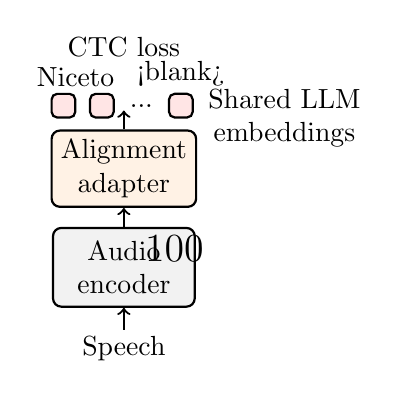
\begin{tikzpicture} [scale=0.8]
        \node(ae) at (0,0) [rectangle, draw=black, fill=gray!10, rounded corners=3pt, thick, minimum width=1.8cm,minimum height=1cm,align=center] {Audio\\encoder};
        \node(freeze) at ([xshift=0.8cm,yshift=0.3cm]ae.center) [rectangle, align=center] {\Large{\ding{100}}};
        \node(fb) at ([yshift=-0.3cm]ae.south) [rectangle, align=center,anchor=north] {Speech};
        \node(aa) at ([yshift=0.3cm]ae.north) [rectangle, draw=black, fill=orange!10, rounded corners=3pt, thick, minimum width=1.8cm,minimum height=0.5cm,align=center,anchor=south] {Alignment\\adapter};
        
        \node(f1) at ([yshift=1.0cm]aa.west) [rectangle, draw=black, fill=red!10, rounded corners=2pt, thick, minimum width=0.3cm, minimum height=0.3cm,align=center,anchor=west] {};
        \node(f2) at ([xshift=0.2cm]f1.east) [rectangle, draw=black, fill=red!10, rounded corners=2pt, thick, minimum width=0.3cm, minimum height=0.3cm,align=center,anchor=west] {};
        \node(f3) at ([xshift=0.075cm]f2.east) [rectangle, draw=white,  thick, align=center,anchor=west] {...};
        \node(f4) at ([xshift=0.075cm]f3.east) [rectangle, draw=black, fill=red!10, rounded corners=2pt, thick, minimum width=0.3cm, minimum height=0.3cm,align=center,anchor=west] {};
        \node(t1) at ([yshift=-0.05cm]f1.north) [rectangle, align=center,anchor=south] {Nice};
        \node(t2) at ([yshift=-0.05cm]f2.north) [rectangle, align=center,anchor=south] {to};
        \node(t4) at ([yshift=-0.05cm]f4.north) [rectangle, align=center,anchor=south] {<blank>};
        \node(se) at ([xshift=0.075cm,yshift=-0.2cm]f4.east) [rectangle, align=center,anchor=west] {Shared LLM\\embeddings};
        \node(ctc) at ([yshift=1.0cm]aa.north) [rectangle, rounded corners=3pt, thick, align=center,anchor=south] {CTC loss};

        
        \draw[->,thick]([yshift=-0.05cm]fb.north)--(ae.south);
        \draw[->,thick](ae.north)--(aa.south);
        \draw[->,thick](aa.north)--([yshift=0.3cm]aa.north);

        
      \end{tikzpicture}
    \end{minipage}
    }
    \subfigure[Shrinking stage]{
    \begin{minipage}[t]{0.45\linewidth}
    \centering
    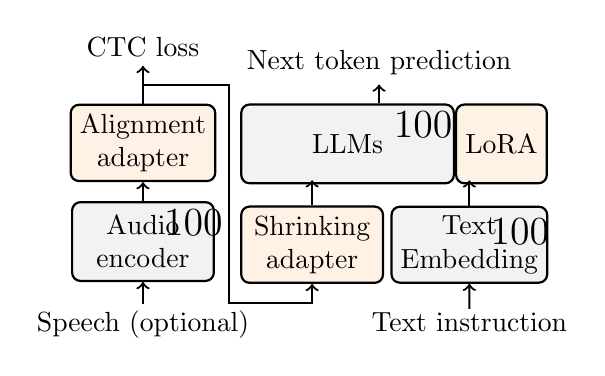
\begin{tikzpicture} [scale=0.8]
        \node(ae) at (0,0) [rectangle, draw=black, fill=gray!10, rounded corners=3pt, thick, minimum width=1.8cm,minimum height=1cm,align=center] {Audio\\encoder};
        \node(freeze) at ([xshift=0.8cm,yshift=0.3cm]ae.center) [rectangle, align=center] {\Large{\ding{100}}};
        \node(fb) at ([yshift=-0.3cm]ae.south) [rectangle, align=center,anchor=north] {Speech (optional)};
        \node(aa) at ([yshift=0.3cm]ae.north) [rectangle, draw=black, fill=orange!10, rounded corners=3pt, thick, minimum width=1.8cm,minimum height=0.5cm,align=center,anchor=south] {Alignment\\adapter};
        \node(ctc) at ([yshift=0.6cm]aa.north) [rectangle,align=center,anchor=south] {CTC loss};
        \node(sa) at ([xshift=0.4cm,yshift=-0.05cm]ae.east) [rectangle, draw=black, fill=orange!10, rounded corners=3pt, thick, minimum width=1.8cm,minimum height=0.5cm,align=center,anchor=west] {Shrinking\\adapter};
        \node(llm) at ([yshift=1.6cm]sa.west) [rectangle, draw=black, fill=gray!10, rounded corners=3pt, thick, minimum width=2.7cm,minimum height=1.0cm,align=center,anchor=west] {LLMs};
        \node(lora) at (llm.east) [rectangle, draw=black, fill=orange!10, rounded corners=3pt, thick, minimum width=1.0cm,minimum height=1.0cm,align=center,anchor=west] {LoRA};
        \node(te) at ([xshift=0.1cm]sa.east) [rectangle, draw=black, fill=gray!10, rounded corners=3pt, thick, minimum width=1.8cm,minimum height=0.5cm,align=center,anchor=west] {Text\\Embedding};
        \node(freeze3) at ([xshift=0.8cm,yshift=0.2cm]te.center) [rectangle, align=center] {\Large{\ding{100}}};
        \node(ti) at ([yshift=-0.3cm]te.south) [rectangle, align=center,anchor=north] {Text instruction};
        \node(freeze2) at ([xshift=1.2cm,yshift=0.3cm]llm.center) [rectangle, align=center] {\Large{\ding{100}}};
        \node(loss) at ([xshift=0.5cm, yshift=0.3cm]llm.north) [rectangle, align=center,anchor=south] {Next token prediction};

        
        \draw[->,thick]([yshift=-0.05cm]fb.north)--(ae.south);
        \draw[->,thick](ae.north)--(aa.south);
        \draw[->,thick](aa.north)--(ctc.south);
        \draw[->,thick](sa.north)--([yshift=0.4cm]sa.north);
        \draw[->,thick](te.north)--([yshift=0.4cm]te.north);
        \draw[->,thick]([yshift=-0.3cm]loss.south)--(loss.south);
        \draw[->,thick]([yshift=-0.1cm]ti.north)--(te.south);

        \draw[->,thick](aa.north)--([yshift=0.3cm]aa.north)--([xshift=0.2cm, yshift=0.3cm]aa.north -| aa.east)--([xshift=0.2cm, yshift=-0.3cm]sa.south -| aa.east)--([yshift=-0.3cm]sa.south)--(sa.south);
      \end{tikzpicture}
    \end{minipage}
    }
    \subfigure[SFT stage]{
    \begin{minipage}[t]{0.20\linewidth}
    \centering
    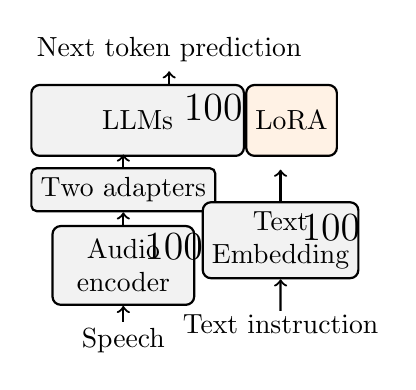
\begin{tikzpicture} [scale=0.8]
        \node(ae) at (0,0) [rectangle, draw=black, fill=gray!10, rounded corners=3pt, thick, minimum width=1.8cm,minimum height=1cm,align=center] {Audio\\encoder};
        \node(freeze) at ([xshift=0.8cm,yshift=0.3cm]ae.center) [rectangle, align=center] {\Large{\ding{100}}};
        \node(fb) at ([yshift=-0.2cm]ae.south) [rectangle, align=center,anchor=north] {Speech};
        \node(aa) at ([yshift=0.2cm]ae.north) [rectangle, draw=black, fill=gray!10, rounded corners=2pt, thick, minimum width=1.8cm,minimum height=0.5cm,align=center,anchor=south] {Two adapters};
        
        \node(llm) at ([yshift=1.1cm]aa.west) [rectangle, draw=black, fill=gray!10, rounded corners=3pt, thick, minimum width=2.7cm,minimum height=0.9cm,align=center,anchor=west] {LLMs};
        \node(lora) at (llm.east) [rectangle, draw=black, fill=orange!10, rounded corners=3pt, thick, minimum width=0.9cm,minimum height=0.9cm,align=center,anchor=west] {LoRA};
        \node(te) at ([xshift=0.1cm,yshift=0.4cm]ae.east) [rectangle, draw=black, fill=gray!10, rounded corners=3pt, thick, minimum width=1.8cm,minimum height=0.5cm,align=center,anchor=west] {Text\\Embedding};
        \node(freeze3) at ([xshift=0.8cm,yshift=0.2cm]te.center) [rectangle, align=center] {\Large{\ding{100}}};
        \node(ti) at ([yshift=-0.4cm]te.south) [rectangle, align=center,anchor=north] {Text instruction};
        \node(freeze2) at ([xshift=1.2cm,yshift=0.2cm]llm.center) [rectangle, align=center] {\Large{\ding{100}}};
        \node(loss) at ([xshift=0.5cm, yshift=0.2cm]llm.north) [rectangle, align=center,anchor=south] {Next token prediction};
       
        \draw[->,thick]([yshift=-0.05cm]fb.north)--(ae.south);
        \draw[->,thick](ae.north)--(aa.south);
        \draw[->,thick](aa.north)--([yshift=0.2cm]aa.north);
        \draw[->,thick](te.north)--([yshift=0.5cm]te.north);
        \draw[->,thick]([yshift=-0.2cm]loss.south)--(loss.south);
        \draw[->,thick]([yshift=-0.1cm]ti.north)--(te.south);
        
      \end{tikzpicture}
    \end{minipage}
    }
      \caption{Training progress of Soundwave. The gray modules are frozen while the orange modules are updated.}
      \label{architecture}
  \end{figure*}

  

\section{Experimental Setup}

\subsection{Dataset}
\label{Sec:dataset}
Our dataset is a snapshot of the Google Play Store, which includes metadata and creatives for 1.3 million apps. This dataset was collected using a Python crawler from January 2023 to November 2023. We deployed an extremely slow crawling rate during this data collection.
For this work, we filtered out and used only the games category, which is more popular among children and as such, the correct content rating matters significantly. During our crawl, the crawler's geo-location was set as Australia (AU) to be consistent in obtaining content rating values of G, PG, M, MA15+, or R18+.

We sorted the selected gaming apps by rank, i.e., sorting in the descending order of number of downloads, star rating count and final star rating number following similar previous work~\cite{seneviratne2015early,rajasegaran2019multi}, and the first 20k games were selected as training and validation sets (80:20 random split) while the next 10k games were selected as the test set. We specifically did not mix the former due to the assumption that more popular apps are well monitored within the community and well maintained by the developers such that the metadata and content ratings information are less noisy than in the rest of the order. Due to the scarcity of games in categories of MA15+ and R18+ within the top 30k, we expanded our search space for them and appended them into train, validation and test sets. For analysis purposes, we created another dataset by including apps with the `Teacher Approved' tag~\cite{teacherAApps}. We report the distribution of apps by content rating across various datasets in Tab.~\ref{tab:dataset_distribution}.


\begin{table}[ht]
    \centering
    \caption{Dataset split and class distribution}
    % \vspace{-0.3cm}
    \label{tab:dataset_distribution}
    \begin{tabular}{l cccc}
    \hline
        & Train & Valid. & Test & Teacher Approved \\
        \hline
        G  & 4,544& 1,139&2,650& 2140\\
        PG & 4,540& 1,130&2,649& 30\\
        M  & 4,530& 1,120&2,648& 2\\
        MA15+ & 2,131& 547&1,796&- \\
        R18+ & 255& 62&255&- \\
        \hline
    \end{tabular}
    % \vspace{-0.3cm}
\end{table}


\begin{figure*}[ht]
    \centering
    \includegraphics[width=\linewidth]{figures/malpractice_examples_v6.pdf}
    \caption{Examples belonging to 1) potential malpractices, and 2) potential disguises. For each app, the image on the left represents the app icon, and on the right is a screenshot. Red * represents app that removed from the Play store after the initial data crawl in 2023.}
    \label{fig:malpractices}
\end{figure*}

\subsection{Implementation Details}
\label{sec:ImplementationDetails}
We use the ViT-B/16 CLIP image encoder as our image backbone for both style and content branches and a frozen RoBERTa backbone in the text encoder branch. The model is pre-trained on eight NVIDIA V100 GPUs for 30 epochs with a minibatch size of 64. We use the Adam optimizer~\cite{kingma2014adam} with learning rate of $10^{-5}$, momentum of $0.9$, and weight decay of $0.02$. The learning rate follows a cosine decay schedule~\cite{loshchilov2016sgdr}, starting from 0 with $10$ warmup epochs and with a final value of $10^{-8}$. We perform a grid search to select the loss coefficients $\lambda$ in Eq.~\ref{eq:finallos} and set it to 5.

\subsection{Content Rating Predictions}
\label{subsec: content rating prediction}

We train a linear classification head to perform content rating predictions based on the previous outputs of image and text embeddings $z_i$ and $z_j$. That is, we propagate them via two separate MLP networks, concatenate the outputs, and then propagate again via another MLP network, followed by softmax classification to identify the prediction class. This stage is shown in Fig.~\ref{fig:model_architecture}(c). As we possess multiple images (app icon and screenshots) for a given app, we take the majority voting for the classification outputs for all of such image and text pairs. Note that we disable back-propagation in all the steps starting from $(i,j)$ up to obtaining $z_i,z_j$ during this classification stage. 

\subsubsection{Performance Metrics}

Due to the persistent class imbalance of our datasets, we report our model's performance in macro and weighted versions of \emph{precision}, \emph{recall} and \emph{F1 scores}. The overall \emph{accuracy} is calculated based on the elements of the principle diagonal of the confusion matrix. Predictions mapping to upper triangular or lower triangular portions of the confusion matrix are undesirable for app users and we later evaluate them in Sec.~\ref{subsec: potential malpractices} as \emph{potential malpractices} and in Sec.~\ref{subsec: potential disguises} as \emph{potential disguises}, respectively. 





% , comparing our results against state-of-the-art image-to-image translation methods
% We evaluate our method through editing experiments conducted on two experiments. In \cref{sec:5.1}, we perform a comparison on image-to-image editing across several datasets. In \cref{sec:5.2}, we extend our evaluation to editable Neural Radiance Fields (NeRF) \cite{mildenhall2021nerf}, demonstrating the efficacy of our approach for 3D image editing and providing a comparative analysis with existing techniques.
% result tables

\section{Results} \label{sec:results}
We evaluate our method through editing experiments conducted on two experiments. In \cref{sec:5.1}, we perform a comparison on image-to-image editing across several datasets. In \cref{sec:5.2}, we extend our evaluation to editable Neural Radiance Fields (NeRF) \cite{mildenhall2021nerf}.

\subsection{Text-guided image editing}
\label{sec:5.1}
\noindent\textbf{Baselines.} To evaluate our method, we conduct comparative experiments against four state-of-the-art image editing models: Prompt-to-Prompt (P2P) \cite{hertzprompt}, Plug-and-Play (PNP) \cite{tumanyan2023plug}, DDS \cite{hertz2023delta}, and CDS \cite{nam2024contrastive}. The implementations of the baselines are carried out by referencing the official source code for each method. More details are provided in \cref{sec:s_implement} of Supplementary Materials.

\noindent\textbf{Qualitative Results.} We present the qualitative results comparing our method with the baselines in \cref{fig:ip2p_qual}. Prompt-to-Prompt (P2P) \cite{hertzprompt} performs image editing after applying DDIM inversion \cite{dhariwal2021diffusion, song2020denoising} to the source image, leading to disregarding the structural components of the source image and following the target prompt excessively. Plug-and-Play (PnP) \cite{tumanyan2023plug} has limitations in object recognition, as seen in the fourth row of Fig.~\ref{fig:ip2p_qual}. The third row of Fig.~\ref{fig:ip2p_qual} demonstrates that DDS \cite{hertz2023delta} and CDS \cite{nam2024contrastive} exhibited limitations, particularly in preserving the structural characteristics of the source image. In contrast, our method successfully edits the image while preserving the structural integrity of the source image.
% exhibit limitations such as failing to maintain the handle length and saddle shape of the bike in the first row and being unable to preserve the structure of the shark in the second row. %Furthermore, as seen in the third and fourth rows, the details in the edited target areas lacked refinement, and in the last row, the color of the source image was not preserved. In contrast, our method successfully edits the image aligning with the target text prompt while preserving the structural integrity of the source image.

\noindent\textbf{Quantitative Results.} 
% We employed two datasets: LAION 5B \cite{schuhmann2022laion} and InstructPix2Pix \cite{brooks2023instructpix2pix}.
% ##ORIGINAL## To measure the identity-preserving performance, we utilize two datasets. First, we collect 250 cat images from the LAION 5B dataset \cite{schuhmann2022laion} based on \cite{nam2024contrastive} for \textit{Cat-to-Others} task. We measure Intersection over Union (IoU) to evaluate how much of the area of the source object has been preserved. Second, we gather 28 images from the InstructPix2Pix (IP2P) dataset \cite{brooks2023instructpix2pix}, which contains the pairs of source and target images and corresponding prompts. We calculate the background Peak-Signal-to-Noise-Ratio (PSNR) to assess how the identity of the source image is preserved after editing. In addition, we use the LPIPS score \cite{zhang2018unreasonable} for each experiment to quantify the similarity between source and target images. The results are presented in \cref{tab:2Dquan}. Our method consistently achieves the lowest LPIPS score across all datasets, indicating that it best preserves the structural semantics of the source images. 
To measure the identity-preserving performance, we utilize two datasets. First, we collect 250 cat images from the LAION 5B dataset \cite{schuhmann2022laion} based on \cite{nam2024contrastive} for \textit{Cat-to-Others} task and measure Intersection over Union (IoU). Second, we gather 28 images from the InstructPix2Pix (IP2P) dataset \cite{brooks2023instructpix2pix}, which contains the pairs of source and target images and corresponding prompts and calculate the background Peak-Signal-to-Noise-Ratio (PSNR). Details of the metrics are provided in Supplementary Materials \cref{sec:s_evalmetric}. In addition, we use the LPIPS score \cite{zhang2018unreasonable} for each experiment to quantify the similarity between source and target images. The results are presented in \cref{tab:2Dquan}. Our method consistently achieves the lowest LPIPS score across all datasets, indicating that it best preserves the structural semantics of the source images. 
% We collect 250 images of cats from the LAION 5B dataset \cite{schuhmann2022laion} based on \cite{nam2024contrastive} for \textit{Cat-to-Others} task and 28 images from the InstructPix2Pix dataset \cite{brooks2023instructpix2pix} following the regulations. To evaluate the images translated by each method, we measure Intersection over Union (IoU) on LAION 5B, which primarily consists of object-focused data. We also measure the background PSNR on InstructPix2Pix to assess the extent to which the source image’s identity is preserved after editing. The results are presented in \cref{tab:2Dquan}. 
% Our method consistently achieves the lowest LPIPS score across all datasets, indicating that it best preserves the structural semantics of the source images. 
\begin{table}[b]
\centering
\resizebox{0.98\columnwidth}{!}{
\small{
\begin{tabular}{c|cc|cc|cc}
\hline
& \multicolumn{2}{c|}{cat2pig} & \multicolumn{2}{c|}{cat2squirrel} & \multicolumn{2}{c}{Ip2p}  \\ 
\hline
\multicolumn{1}{c|}{Metric} & IoU ($\uparrow$) & LPIPS ($\downarrow$) & IoU ($\uparrow$) & LPIPS ($\downarrow$) & PSNR ($\uparrow$) & LPIPS ($\downarrow$) \\ 
\hline
P2P \cite{hertzprompt}& 0.58 & 0.42 & 0.52 & 0.46 & 20.88 & 0.47 \\
PnP \cite{tumanyan2023plug}& 0.55 & 0.52 & 0.53 & 0.52 & 23.81 & 0.39 \\
DDS \cite{hertz2023delta}& 0.69 & 0.28 & 0.65 & 0.30 & 26.02 & 0.24 \\  
CDS \cite{nam2024contrastive}& 0.72 & 0.25 & \textbf{0.71} & 0.26 & 27.35 & 0.21 \\
\hline
\textbf{IDS (Ours)} & \textbf{0.74} & \textbf{0.22} & \textbf{0.71} & \textbf{0.24} & \textbf{29.25} & \textbf{0.19} \\
\hline
\end{tabular}
}
}
\vspace{-5pt}
\caption{\textbf{Quantitative results} for image editing. LPIPS \cite{zhang2018unreasonable} and IoU was measured on LAION 5B \cite{schuhmann2022laion}, while LPIPS and background PSNR was measured on InstructPix2Pix \cite{brooks2023instructpix2pix}.}
\label{tab:2Dquan}
\end{table}




%P2P \cite{hertzprompt}& 0.5798 & 0.4229 & 0.5184 & 0.4605 & 20.88 & 0.4695 \\
%PnP \cite{tumanyan2023plug}& 0.5507 & 0.5191 & ??? & 0.5245 & 23.81 & 0.3882 \\
%DDS \cite{hertz2023delta}& 0.6897 & 0.2838 & 0.6456 & 0.2996 & 26.02 & 0.2398 \\  
%CDS \cite{nam2024contrastive}& 0.7249 & 0.2485 & 0.7054 & 0.2612 & 27.35 & 0.2099 \\

\begin{table}[bh!]
\vspace{-5pt}
\centering
%\scalebox{0.65}
\resizebox{1.0\columnwidth}{!}{
%\small{ %
\begin{tabular}{c|ccc|ccc}
\hline
& \multicolumn{3}{c|}{User Preference Rate (\%)} & \multicolumn{3}{c}{GPT score \cite{peng2024dreambench++}}\\ 
\hline
\multicolumn{1}{c|}{Metric} & Text ($\uparrow$) & Preserving ($\uparrow$) & Quality ($\uparrow$) & Text ($\uparrow$) & Preserving ($\uparrow$) & Quality ($\uparrow$) \\ 
\hline
P2P \cite{hertzprompt}& 11.13 & 4.80 & 8.09 & 5.66 & 5.37 & 5.77 \\
PnP \cite{tumanyan2023plug}& 7.72 & 7.17 & 6.93 & 6.54 & 6.77 & 6.74 \\
DDS \cite{hertz2023delta}& 20.30 & 10.82 & 16.23 & 7.60 & 7.51 & 7.37 \\
CDS \cite{nam2024contrastive}& 17.02 & 16.72 & 17.08 & 8.26 & 8.00 & 8.09 \\ 
\hline
\textbf{IDS (Ours)} & \textbf{43.83} & \textbf{60.49} & \textbf{51.67} & \textbf{8.97} & \textbf{9.00} & \textbf{8.80} \\
\hline
\end{tabular}
}
%}
\vspace{-5pt}
\caption{\textbf{User study and GPT scores}  \cite{peng2024dreambench++} show that our method achieved the highest scores across all questions for image editing.}
\label{tab:Userstudy_GPTscore}
\end{table}
For user evaluation, we present 35 comparison sets for four baselines and our method, gathering responses from 47 participants. Participants are asked to choose the most appropriate image for the following three questions: 1. \textit{Which image best fits the text condition?} 2. \textit{Which image best preserves the structural information of the original image?} 3. \textit{Which image has the best quality for text-based image editing?} 
Additionally, we measure the GPT score using the Dreambench++ \cite{peng2024dreambench++} method, which generates human-aligned assessments for the same questions by refining the scoring into ten distinct levels. As shown in \cref{tab:Userstudy_GPTscore}, our method receives the highest ratings for all questions.
% Furthermore, we ask users to select their favorite image from the baselines in order to gauge their preferences, and we compute the selected ratio in percentage terms.
%While our CLIP score was not significantly higher than other methods, it remained comparable. %Considering the outcomes of both metrics, our model demonstrates an ability to maximally preserve the source image's structure during the editing process while minimally and precisely transforming the regions specified by the target prompt.

% Fig 5.2



%%% [START] NeRF Synthetic data Results 
\begin{figure*}[t] % 2-column
\footnotesize
\centering 
% 1st row
\hspace{-3mm}
\raisebox{0.5in}{\rotatebox{90}{\textbf{Synthetic} \cite{mildenhall2021nerf}}}%
\hspace{3mm}%
\begin{tikzpicture}[x=3.5cm, y=3.5cm, spy using outlines={every spy on node/.append style={thick, draw=red}}]
\node[anchor=south] (FigA) at (0,0) {\includegraphics[trim=0 0 0 0 ,clip,width=1.5in]{Fig./Qual/imgs/3D/ficus/cropped_r_3.png}};
\node[anchor=south, yshift=0mm] at (FigA.north) {\footnotesize Source};
% ->
\draw[->, line width=0.8mm, color=red, shorten >=1pt, shorten <=1pt] ($(FigA.center) + (0.15, -0.18)$) -- ($(FigA.center) + (0, -0.3)$);
\end{tikzpicture}
\hspace{-1mm}
\begin{tikzpicture}[x=3.5cm, y=3.5cm, spy using outlines={every spy on node/.append style={thick, draw=red}}]
\node[anchor=south] (FigD) at (0,0) {\includegraphics[trim=0 0 0 0 ,clip,width=1.5in]{Fig./Qual/imgs/3D/ficus/FPDS_cropped_r_3.png}};
\node[anchor=south, yshift=0mm] at (FigD.north) {\footnotesize \textbf{IDS (Ours)}};
% ->
\draw[->, line width=0.8mm, color=red, shorten >=1pt, shorten <=1pt] ($(FigA.center) + (0.15, -0.18)$) -- ($(FigA.center) + (0, -0.3)$);
\end{tikzpicture}
\hspace{-1mm}
\begin{tikzpicture}[x=3.5cm, y=3.5cm, spy using outlines={every spy on node/.append style={thick, draw=red}}]
\node[anchor=south] (FigC) at (0,0) {\includegraphics[trim=0 0 0 0 ,clip,width=1.5in]{Fig./Qual/imgs/3D/ficus/CDS_cropped_r_3.png}};
\node[anchor=south, yshift=0mm] at (FigC.north) {\footnotesize CDS};
% ->
\draw[->, line width=0.8mm, color=red, shorten >=1pt, shorten <=1pt] ($(FigA.center) + (0.15, -0.18)$) -- ($(FigA.center) + (0, -0.3)$);
\end{tikzpicture}
\hspace{-1mm}
\begin{tikzpicture}[x=3.5cm, y=3.5cm, spy using outlines={every spy on node/.append style={thick, draw=red}}]
\node[anchor=south] (FigB) at (0,0) {\includegraphics[trim=0 0 0 0 ,clip,width=1.5in]{Fig./Qual/imgs/3D/ficus/DDS_cropped_r_3.png}};
\node[anchor=south, yshift=0mm] at (FigB.north) {\footnotesize DDS};
% ->
\draw[->, line width=0.8mm, color=red, shorten >=1pt, shorten <=1pt] ($(FigA.center) + (0.15, -0.18)$) -- ($(FigA.center) + (0, -0.3)$);
\end{tikzpicture}

\vspace{-4pt}

\setulcolor{magenta}
\setul{0.3pt}{2pt}
\centering \textit{``A tree in a brown vase" $\to$ ``A tree in a \ul{blue} vase"} 

\vspace{-2pt}

% 2nd row
\hspace{-3mm}
\raisebox{0.37in}{\rotatebox{90}{\textbf{LLFF} \cite{mildenhall2019local} }}%
\hspace{3mm}%
\begin{tikzpicture}[x=3.5cm, y=3.5cm, spy using outlines={every spy on node/.append style={thick, draw=white}}]
\node[anchor=south] (FigA2) at (0,0) {\includegraphics[trim=0 0 0 0 ,clip,width=1.5in]{Fig./Qual/imgs/3D/autumn/original_image009.jpg}};
\spy [magnification=3, size=0.6in] on ($(FigA2.center) + (0.05, 0.05)$) in node [anchor=south west] at ($(FigA2.south west)$);
\end{tikzpicture}
\hspace{-1mm}
\begin{tikzpicture}[x=3.5cm, y=3.5cm, spy using outlines={every spy on node/.append style={thick, draw=white}}]
\node[anchor=south] (FigD2) at (0,0) {\includegraphics[trim=0 0 0 0 ,clip,width=1.5in]{Fig./Qual/imgs/3D/autumn/FPDS_4032_IMG_3006.jpg}};
\spy [magnification=3, size=0.6in] on ($(FigD2.center) + (0.05, 0.05)$) in node [anchor=south west] at ($(FigD2.south west)$);
\end{tikzpicture}
\hspace{-1mm}
\begin{tikzpicture}[x=3.5cm, y=3.5cm, spy using outlines={every spy on node/.append style={thick, draw=white}}]
\node[anchor=south] (FigC2) at (0,0) {\includegraphics[trim=0 0 0 0 ,clip,width=1.5in]{Fig./Qual/imgs/3D/autumn/CDS_4032_IMG_3006.jpg}};
\spy [magnification=3, size=0.6in] on ($(FigC2.center) + (0.05, 0.05)$) in node [anchor=south west] at ($(FigC2.south west)$);
\end{tikzpicture}
\hspace{-1mm}
\begin{tikzpicture}[x=3.5cm, y=3.5cm, spy using outlines={every spy on node/.append style={thick, draw=white}}]
\node[anchor=south] (FigB2) at (0,0) {\includegraphics[trim=0 0 0 0 ,clip,width=1.5in]{Fig./Qual/imgs/3D/autumn/DDS_4032_IMG_3006.jpg}};
\spy [magnification=3, size=0.6in] on ($(FigB2.center) + (0.05, 0.05)$) in node [anchor=south west] at ($(FigB2.south west)$);
\end{tikzpicture}

% 3rd row
\hspace{-3mm}
\raisebox{0.3in}{\rotatebox{90}{\textbf{Depth Map}}}%
\hspace{3mm}%
\hspace{0mm}
\begin{tikzpicture}[x=3.5cm, y=3.5cm, spy using outlines={every spy on node/.append style={thick, draw=white}}]
\node[anchor=south] (FigA3) at (0,0) {\includegraphics[trim=0 0 0 0 ,clip,width=1.5in]{Fig./Qual/imgs/3D/autumn/depth_map/original_depth_088.jpg}};
\end{tikzpicture}
\hspace{-1mm}
\begin{tikzpicture}[x=3.5cm, y=3.5cm, spy using outlines={every spy on node/.append style={thick, draw=white}}]
\node[anchor=south] (FigD3) at (0,0) {\includegraphics[trim=0 0 0 0 ,clip,width=1.5in]{Fig./Qual/imgs/3D/autumn/depth_map/FPDS_depth_088.jpg}};
\end{tikzpicture}
\hspace{-1mm}
\begin{tikzpicture}[x=3.5cm, y=3.5cm, spy using outlines={every spy on node/.append style={thick, draw=white}}]
\node[anchor=south] (FigC3) at (0,0) {\includegraphics[trim=0 0 0 0 ,clip,width=1.5in]{Fig./Qual/imgs/3D/autumn/depth_map/CDS_depth_088.jpg}};
\end{tikzpicture}
\hspace{-1mm}
\begin{tikzpicture}[x=3.5cm, y=3.5cm, spy using outlines={every spy on node/.append style={thick, draw=white}}]
\node[anchor=south] (FigB3) at (0,0) {\includegraphics[trim=0 0 0 0 ,clip,width=1.5in]{Fig./Qual/imgs/3D/autumn/depth_map/DDS_depth_088.jpg}};
\end{tikzpicture}

\vspace{-1pt}
\centering \textit{``The green leaves" $\to$ ``\ul{Yellow and red} leaves in \ul{autumn}"} 

\vspace{-5pt}
\caption{\textbf{Qualitative results on Synthetic 360$^\circ$ and LLFF datasets.} IDS outperforms the baselines by preserving the structural consistency of the source image and maintaining the integrity of regions that should remain unchanged, while precisely editing only the areas specified by the target prompt. Furthermore, comparisons of the depth map results also highlight the superior consistency of our method over other baseline models.}
\label{fig:ficus_qual}
\end{figure*}
% \vspace{-10pt}
\subsection{Editing NeRF}
We conduct experiments involving 3D rendering of edited images to demonstrate the effectiveness of our method in maintaining structural consistency. This approach is particularly relevant as consistency has an even greater impact on outcomes in 3D environments.

\label{sec:5.2}

\noindent\textbf{Datasets.} We evaluated our method on widely used NeRF datasets: Synthetic NeRF \cite{mildenhall2021nerf} and LLFF \cite{mildenhall2019local}. Since NeRF datasets have no given pairs of source and target prompts, we manually composed image descriptions.
%, such as the source prompt ``A tree in a brown vase" and its corresponding target prompt ``A tree in a blue vase" as shown in \cref{fig:ficus_qual}.

\noindent\textbf{Qualitative Results.} \cref{fig:ficus_qual} illustrates the qualitative results of our method compared with NeRF editing baselines. In the first row, the target prompt specifies a precise part of the image for fine-grained editing. DDS \cite{hertz2023delta} and CDS \cite{nam2024contrastive} fail to differentiate and edit the specific area. At the same time, our method accurately identifies the region indicated by the target prompt in the image and performs detailed editing exclusively on that part. 
The second row demonstrates a scenario in which the target prompt is designed to edit the mood of the image. Our approach adjusts the colors associated with ``autumn" and ``leaves" throughout the image while maintaining consistency in the ``trunk" whereas DDS and CDS also changed the ``trunk". In terms of depth maps, our method generates clean depth maps with minimal noise after image editing, whereas DDS and CDS introduce noticeable noise into the depth maps.

%the overall mood of the image on the LLFF dataset \cite{mildenhall2019local}
 % give an attention solely on following the target prompt during editing, leading to unintended alterations of parts that should remain unchanged.
 % Comparing the NeRF depth maps with baselines, 
% \cref{fig:ficus_qual} illustrates the qualitative results of our method compared with NeRF editing baselines such as DDS \cite{hertz2023delta} and CDS \cite{nam2024contrastive}. In the first row, the target prompt specifies a precise part of the image for fine-grained editing on the Synthetic NeRF dataset \cite{mildenhall2021nerf}. Our method accurately identifies the region indicated by the target prompt in the image and performs detailed editing exclusively on that part. In contrast, DDS and CDS fail to differentiate and edit the specific area; they erroneously edit not only the ``vase" but also the ``soil", resulting in inappropriate edits. The second row demonstrates a scenario in which the target prompt is designed to edit the overall mood of the image on the LLFF dataset \cite{mildenhall2019local}, further highlighting the strengths of our method. Our approach adjusts the colors associated with ``autumn" and ``leaves" throughout the image while maintaining consistency in the ``trunk", which should be preserved from the source image. However, DDS and CDS focus solely on following the target prompt during editing, leading to unintended alterations of parts that should remain unchanged. Additionally, comparing the NeRF depth maps with baselines, our method generates clean outputs with minimal noise after image editing, whereas DDS and CDS introduce noticeable noise into the depth maps. 
% \vspace{-10pt}
% % Table for CLIP score
% \begin{table}[H]
% \centering
% \resizebox{0.9\columnwidth}{!}{
% \begin{tabular}{ccc}
% \toprule
% Metric & CLIP \cite{radford2021learning} score ($\uparrow$) & User Preference Rate ($\uparrow$) \\
% \midrule
% CDS \cite{nam2024contrastive}& $0.1597$ & $22.7$ \\
% DDS \cite{hertz2023delta}& $0.1596$ & $??$ \\
% \textbf{FPDS (ours)} & $\mathbf{0.1626}$ & $\mathbf{??}$ \\
% \bottomrule
% \end{tabular}
% }
% \caption{\textbf{Quantitative results of NeRF editing} comparing our method with other baselines for CLIP score and User Preference Rate on the NeRF LLFF dataset \cite{mildenhall2019local}. Higher CLIP scores and User Preference Rates indicate better performance.}
% \label{tab:Nerfclip}
% \end{table}
\begin{table}[thb!]
\centering
\resizebox{0.95\columnwidth}{!}{
\begin{tabular}{c|c|ccc}
\hline
\multirow{2}{*}{Metric} & \multirow{2}{*}{CLIP \cite{radford2021learning}  ($\uparrow$)} & \multicolumn{3}{c}{User Preference Rate (\%)} \\ 
\cline{3-5}
& & Text ($\uparrow$) & Preserving ($\uparrow$) & Quality ($\uparrow$) \\ 
\hline
DDS \cite{hertz2023delta}& 0.1596 & 36.88 & 28.37 & 32.62 \\
CDS \cite{nam2024contrastive}& 0.1597 & 22.70 & 23.40 & 21.28 \\
\hline
\textbf{IDS (Ours)} & \textbf{0.1626} & \textbf{40.42} & \textbf{48.23} & \textbf{46.10} \\
\hline
\end{tabular}
}
\caption{\textbf{Quantitative results of NeRF editing} with respect to CLIP score and User Preference Rate. IDS demonstrates superior quantitative performance compared to the baselines.}
\label{tab:Nerfclip}
\end{table}


\noindent\textbf{Quantitative Results.} Based on edited images, we performed 3D rendering and subsequently conducted quantitative evaluations provided in \cref{tab:Nerfclip}. To assess whether the edited 3D images are precisely aligned with the target prompts, we measured the CLIP \cite{radford2021learning} scores at 200k iterations of training on the LLFF dataset. We additionally present a user evaluation conducted under the same setup in \cref{sec:5.1}. Consistent with the trends observed in the qualitative results, our method demonstrates superior performance in the quantitative evaluations compared to other baselines.
%To demonstrate the effectiveness of our method in maintaining structural consistency during image editing and correcting errors progressively throughout training, we also conduct experiments involving 3D rendering of edited images. This approach is particularly relevant as consistency has an even greater impact on outcomes in 3D environments.


\section{Result Analysis}

In this section, we analyse the results and predictions of our method from the perspective of the mobile app ecosystem. First, we observe how deviated the text and visual data are compared to natural language and text. Next, we present interesting findings among the lower and upper triangular parts of the confusion matrix (i.e., apps having a lower or higher content rating than our predictions). 


\subsection{Image-text Cross Attention}
\begin{figure}[ht]  
    \centering
    \includegraphics[width=0.97\linewidth]{figures/vis_ca_module.pdf}
    \caption{Visualisation of image patches attending to text tokens in the custom cross-attention layer.}
    \label{fig:ca_visualized}
\end{figure}

In Sec.~\ref{ssec:cross attention}, we discussed how our image-text cross attention (CA) design allows every patch of the content image to attend over all tokens in the text input sequence. Also, for each image patch, there are 12 attention heads running in parallel. Therefore, to qualitatively measure how the CA happens, we select attention-heads of the first layer as lower layers are often associated with broader attention~\cite{vig_2019_multiscale}. Then, for each image patch, we select the tokens with the highest numerical attention values after excluding some stop-word and punctuation mark-related tokens. In Fig.~\ref{fig:ca_visualized}, we visualise the highly attended words in a given input image portion for some example images. An image portion is a collection of consecutive patches which we select as a region of interest; for example, the patches outlining the gun in Fig.~\ref{fig:ca_visualized} (d) or the heart in Fig.~\ref{fig:ca_visualized} (a). The results show that mobile app ecosystem-related tokens such as `simulator', `game', `upgrade', and `developers' are now attended by the image patches, even though those words cannot be identified by observing the image in a general context. Furthermore, the tokens representing target audiences such as `kids', `children' and `girls' are now attended. This further demonstrates how our model has been able to reduce the gap between visual data and textual data in the mobile app domain.

\subsection{Predictions in the Wild}

When our classifier is applied to the test set containing 10,000 gaming apps, two interesting cases emerge, i.e., apps with a higher or lower labelled rating than our model's predictions. These two scenarios lead to potential  \emph{``malpractices"} and \emph{``disguises"} that are important from a content safety point of view. 

\subsubsection{Potential malpractices}
\label{subsec: potential malpractices}

When our method predicts a class label that is higher than the developer-defined label, we characterise such examples as possible malpractices (i.e., having a lower content rating than what the app is supposed to have). Occurrences belonging to this category could be identified along the horizontal axis of the confusion matrix, on the right-hand side to the diagonal. This is more observed in the G category as any higher prediction, such as PG, M, MA15+, and R18+, raises a concern. As we go higher in prediction classes, the possibilities for malpractices decrease, and therefore, the R18+ category is not susceptible to malpractices. 

We manually evaluated 350 apps with predicted labels that were two classes or more higher than the true label (e.g., prediction [M, MA15+ or R18+] when the true label is [G]) and identified 62 (17.7\%) of them as potential malpractices (i.e., possible content rating violations). \textit{Also, we highlight that at the time of writing, 14 of them were removed from Play Store, and 20 of them were increased to a higher rating class compared to the time we crawled the dataset. While we can't be exactly sure why these 14 apps were removed from  Google Play Store, previous work has reported that Google take down apps violating their content policies~\cite{seneviratne2015early}.} 

We highlight ten exemplary instances that are potentially linked to malpractices in Fig.~\ref{fig:malpractices} (1). Examples (a) and (b) both represent gambling-related games rated [G] that would at least require a rating of [PG]. Example (c) depicts shooting and gun usage, again not suitable for a general audience. (e) and (j) contain images more suited for an [MA15+] audience, and (d) and (f) entertain visual and textual cues strongly related to illegal substances that require a rating higher than [PG]. (g) and (h) contain images with horror themes, blood and intense cartoon or fantasy violence which are more suited for [MA15+] audience. These examples suggest that our model can flag potential content malpractices in the app ecosystem.


\subsubsection{Potential disguises}
\label{subsec: potential disguises}

Apps belonging to higher content ratings are likely not to conduct malpractices, but alarmingly, they could be disguised as a lower-rated app and, as a consequence, could attract an unsuitable audience to the app.  
As an example, an R18+ app consisting of cartoonish images and not-so-alarming textual data could attract underage audiences due to their natural tendency for curiosity and their interest in cartoons. From the developer's perspective, they comply with the content policies and applicable laws. However, in such cases, we argue that at least the textual description must contain information such that someone (e.g., a parent or a guardian) who misses the content rating label should be able to figure out the app's purpose and functionality independently. We define this category as possible disguises. R18+ is more vulnerable to disguises that can be identified horizontally left to the diagonal of the confusion matrix. Being the lowest content rating, category [G] is not susceptible to disguises. We checked 131 samples that were predicted [G, PG, M] when the true class was [R18+], and 203 samples predicted [G] when the true class was [MA15+] and observed $\sim$9.3\% of them to be possible disguises.

We demonstrate some of such examples in Fig.~\ref{fig:malpractices}(2). App represented by (a) is an app rated for [PG] and our method predicts even lower as [G]. Observing the images, it is evident their content is sexual in nature despite the cartoonish theme. In our test dataset, the average rating for an app with such sexualised imagery is [MA15+]. 
Note that in this category, our model is likely to predict a lower rating as the images or text is not suggestive of requiring high ratings. Due to such examples being rare, our model does not know how to predict them correctly, yet we still can automatically identify them based on our off-to-left-diagonal results, as explained before. Apps (b, e, g) and (i), though rated for [MA15+] and higher based on a storyline related to a `fashion and makeup', is likely to attract a younger audience due to the visual appearance similar to the majority of [PG] rated \emph{Dress up} games. A similar interpretation can be given to [M] rated examples (c, h), which are too cartoonish yet contain images related to mature audiences, such as pregnancy. Furthermore, (f) and (j) are rated as [MA15+], which contains appealing games for young audience. Despite measures such as \emph{Not designed for children} tagging is available in Google Play~\cite{notdisgisechil.} to safeguard users, it doesn't appear to be used by many developers. 

\subsubsection{Unverifiable apps} 
\label{subsec: unverifiable_apps}

\begin{figure}[ht]  
    \centering
    \includegraphics[width=0.97\linewidth]{figures/unverifiables.pdf}
    \caption{Examples of unverifiable apps with developer defined content rating descriptors.}
    \label{fig:unverifiable_apps}
\end{figure}
We further highlight discrepancies in content rating declarations, as illustrated in Fig.~\ref{fig:unverifiable_apps}. These noisy instances represent cases where we could not manually verify the developer-assigned ratings based on the app’s available metadata, visuals, or descriptions. The app in (a) is rated as [M] with descriptors indicating simulated gambling, online interactivity, and in-game purchases. However, compared to similar games in the dataset, it does not display any visual cues or textual descriptions to justify such a rating. Therefore, the absence of gambling graphics or explicit mention of gambling mechanics justifies the predicted rating of [G].
Similarly, app (b) and (c) fail to reflect sensitive content such as sexualised imagery and strong violence in app creatives. Hence, in all these cases, our model predicted a lower rating than the original rating. While it may not be explicitly illegal to omit sensitive descriptors from app screenshots or descriptions, missing descriptors in visuals hinder the user's ability to make informed decisions, leading to unwanted downloads or unexpected experiences and children and vulnerable users may unintentionally be exposed to harmful or age-inappropriate content.


\subsubsection{Teacher Approved (TA) Apps}

\begin{figure}[ht]  
    \centering
    \includegraphics[width=0.97\linewidth]{figures/teacher_approved_v2.pdf}
    \caption{Examples of teacher-approved apps with incorrect content ratings - A section of the app description is quoted and * indicates this app is no longer available.}
    \label{fig:teacher_apps}
\end{figure}


Google Play has deployed the `teacher approved' apps based on consultations with experts to determine the suitability for kids, and especially the age appropriateness~\cite{teacherAApps}. Hence, these apps are likely to be more content appropriate as per the rating labelling. However, after analysing 2,172 TA apps, we found that our model predictions deviate from the declared content rating classifications, with 10.4\% of them being flagged for potential malpractices. Among them, 92\% of the instances were flagged as requiring [PG] despite being declared as [G]. Further evaluating their continuity, within a time span of nine months, we observed that 34.5\% of apps that were classified as potential malpractices have been removed from the Play Store. On the contrary, only 27.4\% of correctly predicted apps were removed, which is lower compared to the deletion rate of apps identified with malpractices.
We further discuss why app removal rate can be a proxy measure of content policy violations in the next subsection. 


As depicted in Fig.~\ref{fig:teacher_apps} we manually verified a portion of apps flagged before as malpractices based on the available metadata and identified that nine apps are likely to be not suitable for children despite being tagged as TA. 
The presence of violence (Fig.~\ref{fig:teacher_apps}a), horror themes (Fig.~\ref{fig:teacher_apps}b) or online multiplayer interactions (Fig.~\ref{fig:teacher_apps}d) were the main reasons we identified behind these content rating discrepancies. 
The example in Fig.~\ref{fig:teacher_apps} c highlights a contradiction in the app's description, which mandates parental presence, despite the app being labeled as [G] in the Play Store.
\textit{Overall, the presence of these practices among `teacher approved' apps is alarming. It shows that even manually verified apps are not immune to content rating malpractices, and further rigour is required in app vetting.}


\begin{figure}[ht]    
    \centering
    \includegraphics[width=0.97\linewidth]{figures/app_deletion_rate_.pdf}
    \caption{App deletion rates w.r.t number of downloads.}
    \label{fig:app_deletion}
   % \vspace{-0.3cm}
\end{figure}


\subsubsection{App Deletion Rate}

An app can be discontinued in Google Play for two reasons: the developer could discontinue the app~\cite{denipitiyage2024detecting}, or Google could remove the app for violating its policies~\cite{2023gplypolicyviolation}. As a result, an app being removed from Google Play can be used as an indication of a possible violation of Google Play policies.

To this end, we used 15,985 apps that are gathered from the test set (10,000 apps: c.f. Sec.~\ref{Sec:dataset}) added with 5,985 apps with lower downloads (download count $<$ 100,000 - to account for a better distribution as our test set consists of top apps only). Next, we attempted to re-crawl these apps to check whether they were still there in Google Play. Overall, we found 45.7\% of apps identified as having malpractices, 39.1\% of apps that predicted to be disguises were removed within the time span of nine months. In comparison only  29.1\% of apps that correctly predicted were removed.


In Fig.~\ref{fig:app_deletion}, we show the percentage of apps that we found as deleted according to the download numbers and the predictions of our classifier. At all download ranges apart from `$<$ 100', we notice that apps we classified as potential malpractices have a higher deletion rate than apps we classified as correct. Similar values of `$<$~100' category can be explained by less attention and consequently fewer complaints received on those apps for Google to action.

On the other hand, apps classified as disguises are likely not to be removed as malpractices, as they are unlikely to be noticed or complained about by an average audience. Notably, apps flagged as disguises with more than 1M downloads are far less likely to be removed as the number of apps with a higher content rating label (e.g., MA15+, R18+) are not frequent among the apps. 



This work presented \ac{deepvl}, a Dynamics and Inertial-based method to predict velocity and uncertainty which is fused into an EKF along with a barometer to perform long-term underwater robot odometry in lack of extroceptive constraints. Evaluated on data from the Trondheim Fjord and a laboratory pool, the method achieves an average of \SI{4}{\percent} RMSE RPE compared to a reference trajectory from \ac{reaqrovio} with $30$ features and $4$ Cameras. The network contains only $28$K parameters and runs on both GPU and CPU in \SI{<5}{\milli\second}. While its fusion into state estimation can benefit all sensor modalities, we specifically evaluate it for the task of fusion with vision subject to critically low numbers of features. Lastly, we also demonstrated position control based on odometry from \ac{deepvl}.
\section{Acknowledgment}
This research was supported by the Australian Government through the Australian Research Council’s Discovery Projects funding scheme (Project ID DP220102520).

% \newpage
\bibliographystyle{IEEEtran}
\bibliography{biblio}

\begin{IEEEbiography}[{\includegraphics[width=1in,height=1.25in,clip,keepaspectratio]{bio_pics/dewni.jpeg}}]{Dishanika Denipitiyage}
	received her Bachelors degree in Electronic and Telecommunication Engineering from University of Moratuwa, Sri Lanka in 2020. She is currently working toward the PhD degree with the School of Computer Science, University of Sydney, Australia. She worked as a Senior software engineear at SenzMate (Pvt) Ltd, Sri Lanka in 2022 and as a Visiting Research Intern at Singapore University of Technology and Design (SUTD), Singapore in 2017. Her research interests include Self-Supervised Learning and Multi-Modal learning.
\end{IEEEbiography}

\vskip -3\baselineskip plus -1fil
\vspace{8mm}

\begin{IEEEbiography}[{\includegraphics[width=1in,height=1.5in,clip,keepaspectratio]{bio_pics/bhanuks.jpeg}}]{Bhanuka Silva}
received his Bachelors degree in Electronic and Telecommunication Engineering (First Class Hons.) from University of Moratuwa, Sri Lanka in 2020. He also worked as a Visiting Research Intern at Data61-CSIRO, Brisbane in 2018 and is currently a doctoral student at the University of Sydney and his current research focuses on conducting privacy compliance checks in mobile app eco-systems by leveraging state-of-the art natural language processing techniques.
\end{IEEEbiography}

\vskip -3\baselineskip plus -1fil
\vspace{8mm}

\begin{IEEEbiography}[{\includegraphics[width=1in,height=1.25in,clip,keepaspectratio]{bio_pics/kavishka.jpeg}}]{Kavishka Gunathilaka}
is a B.Sc. Eng. undergraduate in the Department of Computer Science and Engineering of the University of Moratuwa, Sri Lanka. He also worked as a Research Affiliate at the University of Sydney in 2023. His primary research interests include machine learning, data 
science, and artificial intelligence.
\end{IEEEbiography}

\vskip -3\baselineskip plus -1fil
\vspace{8mm}

\begin{IEEEbiography}[{\includegraphics[width=1in,height=1.25in,clip,keepaspectratio]{bio_pics/ssenevirathne.png}}]{Suranga Seneviratne}
is a Senior Lecturer in Security at the School of Computer Science, The University of Sydney. He received his Ph.D. from the University of New South Wales, Australia in 2015. His current research interests include privacy and security in mobile systems, AI applications in security, and behavior biometrics. Before moving into research, he worked nearly six years in the telecommunications industry in core network planning and operations. He received his bachelor degree from University of Moratuwa, Sri Lanka in 2005.
\end{IEEEbiography}
%\vspace{-4.2cm}

\vskip -2\baselineskip plus -1fil
\vspace{8mm}

\begin{IEEEbiography}[{\includegraphics[width=1in,height=1.25in,clip,keepaspectratio]{bio_pics/amahanti.jpeg}}]{Anirban Mahanti}'s technical expertise is at the intersection of computer networking, data science, and machine learning. Anirban earned his Ph.D. in Computer Science from the University of Saskatchewan, Canada, in 2003, his MSc in Computer Science in 1999, and his BE in Computer Science and Engineering from the Birla Institute of Technology, India, in 1993. He is currently an Honorary Senior Research Fellow at the University of Sydney.
\end{IEEEbiography}
\vskip -2\baselineskip plus -1fil
\begin{IEEEbiography}[{\includegraphics[width=1in,height=1.25in,clip,keepaspectratio]{bio_pics/aruna.jpeg}}]{Aruna Seneviratne}
(Senior Member, IEEE) is currently a foundation professor of telecommunications with the University of New South Wales, Sydney, Australia, where he holds the Mahanakorn chair of telecommunications. He was with a number of other universities in Australia, UK, and France, as well as industrial organizations, including Muirhead, Standard Telecommunication Labs, Avaya Labs, and Telecom Australia (Telstra). He held visiting appointments with INRIA, France. His research inter- ests include physical analytics, technologies that enable applications to interact intelligently and securely with their environment in real time. Recently, his team has been working on using these technologies in behavioural biometrics, optimizing the performance of wearables, and IoT system verification. He was the recipient of several fellowships, including one at British Telecom and one at Telecom Australia Research Labs.
\end{IEEEbiography}

\vskip -2\baselineskip plus -1fil
\vspace{8mm}

\begin{IEEEbiography}[{\includegraphics[width=1in,height=1.25in,clip,keepaspectratio]{bio_pics/schawla.png}}]{Sanjay Chawla}
is Research Director of QCRI’s Data Analytics department. Prior to joining QCRI, Dr. Chawla was a Professor in the Faculty of Engineering and IT at the University of Sydney. From 2008-2011, he also served as the Head (Department Chair) of the School of Information Technologies. He was an academic visitor at Yahoo! Research in 2012. He received his PhD from the University of Tennessee (USA) in 1995. His research is in data mining and machine learning with a specialization in spatio-temporal data mining, outlier detection, class imbalanced classification, and adversarial learning. 
\end{IEEEbiography}

\end{document}

